\documentclass[cnatzke_thesis_proposal.tex]{subfiles}
\begin{document}

\chapter{The GRIFFIN Spectrometer at TRIUMF}

%%%%%%%%%%%%%%%%%%%%
\subsection{TRIUMF Rare Isotope Beam Facility}
%%%%%%%%%%%%%%%%%%%%
\begin{figure}[H]
  \begin{center}
    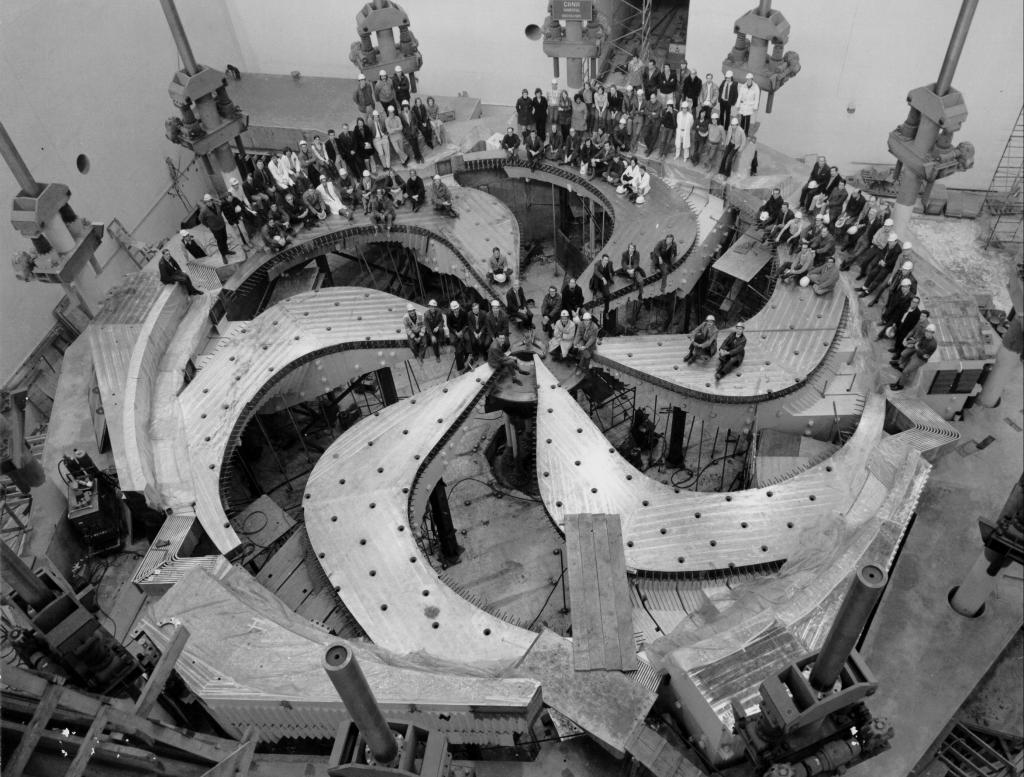
\includegraphics[width=0.95\linewidth]{triumf_cyclotron_construction_1972.jpg}
  \end{center}
  \caption{TRIUMF cyclotron during initial construction (1972) - Figure courtesy of TRIUMF.}
  \label{fig:triumf_cyclotron_1972}
\end{figure}

The proposed experiment will be performed at Canada's national laboratory for nuclear and particle physics, TRIUMF. 
TRIUMF is located in Vancouver, British Columbia, Canada and was established in 1968 by three universities, Simon Fraser University, the University of British Columbia (UBC), and the University of Victoria, as an experimental facility to meet needs the three universities could not individually provide. 
Since then the science program has grown to include nuclear physics, particle physics, molecular and material science, and nuclear medicine while providing research infrastructure and tools too large or complex for a single university to build, operate, or maintain. 
TRIUMF houses the world's largest cyclotron \cite{dilling_isac_2014} capable of accelerating protons up to 520 MeV before they are delivered to the experimental halls, via one of four beam lines, for direct use or to create secondary radioactive isotope beams of pions, muons, or radioactive isotopes. 
This work uses the GRIFFIN spectrometer housed in the ISAC-I experimental hall located on the TRIUMF-ISACI experimental hall. 

%%%%%%%%%%%%%%%%%%%%
\subsection{The GRIFFIN Spectrometer}
%%%%%%%%%%%%%%%%%%%%

\begin{center}
\begin{figure}[H]
  \begin{center}
    \includegraphics[scale=.18]{isac_i_facility.png}
  \end{center}
  \caption{Schematic view of the TRIUMF-ISAC facility \cite{Dilling2014}, including the target ion-source, the high resolution mass separator, and various detection stations.}
  \label{fig:ISAC_HALL}
\end{figure}
\end{center}

Large scale detector arrays for $\gamma$-ray measurements provide a powerful and robust tool for studying unstable nuclei through radioactive decay and nuclear spectroscopy at radioactive ion beam facilities \cite{garnsworthy_griffin_2019}. 
The Gamma-Ray Infrastructure For Fundamental Investigations of Nuclei (GRIFFIN) is a high-efficiency $\gamma$-ray spectrometer composed of sixteen large-volume clover-type High Purity Germanium (HPGe) detectors located in the ISAC-I experimental hall at TRIUMF. 
The detectors are arranged to cover sixteen of the eighteen faces of a rhombicuboctahedron with the front faces of the detectors able to be set 110 or 145 mm from the beam implantation location at the centre of the array. 


The TITAN groups' experimental setup consists of 5 traps, Cooler Penning Trap (CPET), Measurement Penning Trap (MPET), Multi-reflection Time of Flight Mass Spectrometer (MR-TOF-MS), Electron Beam Ion Trap (EBIT) as well as a Radio Frequency Quadapole (RFQ) linear Paul trap which functions as a cooler and buncher.  
These systems can operate alone or in conjunction such as where the RFQ cools and bunches the beam before passing it off to the MR-TOF-MS.  
From there the MR-TOF-MS can clean the beam for a specific mass to great precision before passing it off to the EBIT for further charge breeding and possible injection into MPET or CPET.  
The ability for TITAN to combine instruments for purification and trapping gives it a unique ability to probe fundamental nuclear and atomic properties.

\subsection{The TITAN Electron-Beam Ion Trap (EBIT)}

\begin{figure}[H]
  \begin{center}
    \includegraphics[scale=.3]{EBIT1.png}
  \end{center}
  \caption{Schematic view of EBIT}
  \label{fig:EBIT_CUTOUT}
\end{figure}

The electron-beam ion trap serves to generate highly-charged ions (HCIs) by means of an intense electron beam causing electron-impact ionization and trap them via electro-magnetic fields.  
The TITAN EBIT was built at the Max-Planck-Institute for Nuclear Physics (MPI-K) in Heidelberg from 2004-2006 \cite{TITAN_EBIT_2010}. 
The EBIT uses a very strong (near 6T) magnetic field generated by pair of coils in a Helmholtz geometry to compress the electron beam creating a very high current density to facilitate the electron-impact ionization.  
The HCIs are trapped in the axial direction by a symmetric electrostatic quadrupole potential well which is achieved via applying a potential to the EBIT's drift tubes.  
Radial confinement is handled by the electron-beam space-charge potential along with the previously mentioned strong magnetic field \cite{TITAN_EBIT_2010}.

\begin{figure}[H]
  \begin{center}
    \includegraphics[scale=.3]{ebit_schematic.png}
  \end{center}
  \caption{Schematic view of EBIT \cite{PALFFY_THESIS}}
  \label{fig:schematic_ebit}
\end{figure}

(Fig. \ref{fig:schematic_ebit} )
**DESCRIBE  THRESHOLD CHARGE BREEDING**
For a Penning trap the relative precision of the mass measurement is proportional to the charge state of the ion which can be approximated via (Eq. \ref{eq:ebit_resolving_power} \cite{TITAN_EBIT_2010})


\begin{equation}
  \frac{\delta m}{m} \propto \frac{m}{qB} \frac{1}{T_{RF}} \frac{1}{\sqrt{N}}
  \label{eq:ebit_resolving_power}
\end{equation}

here $T_{RF}$ represents the excitation time in the magnetic field $B$ with $N$ representing the number of measurements.  From this it is clear the powerful benefits inherent in using an EBIT to further charge breed ions before passing them to a Penning trap \cite{TITAN_EBIT_2010}.

The time to breed to a specific charge state is given by (Eq. \ref{eq:ebit_stripping_time})
\begin{equation}
  \tau_{i}(q) = \sum_{q'=0}^{q-1}\langle n_e v_e \sigma^{I}_{q', q'+1} \rangle^{-1}
  \label{eq:ebit_stripping_time}
\end{equation}

where $\sigma^{I}_{q', q'+1}$ is the cross section for single ionization and $n_e v_e$ is equal to the current density divided by the elementary charge $\frac{j_e}{e}$ \cite{SPRINGER_1997}.


\end{document}
